% $Header: /cvsroot/latex-beamer/latex-beamer/solutions/conference-talks/conference-ornate-20min.en.tex,v 1.6 2004/10/07 20:53:08 tantau Exp $

\documentclass{beamer}

\mode<presentation>
{
%  \usetheme{Hannover}
\usetheme[width=0.7in]{Hannover}
% or ...

  \setbeamercovered{transparent}
  % or whatever (possibly just delete it)
}
\usepackage{longtable}
\usepackage{booktabs}
%\usepackage{qtree}

\usepackage[english]{babel}
% or whatever

\usepackage[latin1]{inputenc}
% or whatever

\usepackage{times}
%\usepackage[T1]{fontenc}
% Or whatever. Note that the encoding and the font should match. If T1
% does not look nice, try deleting the line with the fontenc.
%\usepackage{logictheme}

\usepackage{multirow}
\usepackage{totpages}
\usepackage{hyperref}
\usepackage{booktabs}
\usepackage[round]{natbib}

\usepackage{listings}
\lstset{frame=none, showstringspaces=false, basicstyle=\ttfamily\bfseries\footnotesize,
  xleftmargin=-8mm,language=Haskell,breaklines=true}

\usepackage{tikz}
\usetikzlibrary{positioning}
\usepackage{viking}

\usepackage{pifont}
\usepackage{amsmath,amsfonts,xspace,xcolor,url}
\newcommand{\cross}{\ding{55}}

\newcommand{\blt}{- } %used for bullets in a list

\newcounter{datadefnum} %Datadefinition Number
\newcommand{\ddthedatadefnum}{DD\thedatadefnum}
\newcommand{\ddref}[1]{DD\ref{#1}}

\newcommand{\colAwidth}{0.1\textwidth}
\newcommand{\colBwidth}{0.8\textwidth}

\renewcommand{\arraystretch}{1.1} %so that tables with equations do not look crowded

\pgfdeclareimage[height=0.7cm]{logo}{McMasterLogo}
\title[\pgfuseimage{logo}] % (optional, use only with long paper titles)
{Drasil in a Nutshell}

%\subtitle
%{Include Only If Paper Has a Subtitle}

\author[Slide \thepage~of \pageref{TotPages}] % (optional, use only with lots of
                                              % authors)
{Spencer Smith, Jacques Carette}
% - Give the names in the same order as the appear in the paper.
% - Use the \inst{?} command only if the authors have different
%   affiliation.

\institute[McMaster University] % (optional, but mostly needed)
{
  Computing and Software Department\\
  Faculty of Engineering\\
  McMaster University
}
% - Use the \inst command only if there are several affiliations.
% - Keep it simple, no one is interested in your street address.

\date[Jan 12, 2016] % (optional, should be abbreviation of conference name)
% {CAIMS 2017, Third Canadian Symposium in Numerical Analysis and Scientific
% Computing (CSNASC): Simulation, July 18, 2017}
% - Either use conference name or its abbreviation.
% - Not really informative to the audience, more for people (including
%   yourself) who are reading the slides online

\subject{computational science and engineering, software engineering, software
  quality, literate programming, software requirements specification, document
  driven design}
% This is only inserted into the PDF information catalog. Can be left
% out. 

% If you have a file called "university-logo-filename.xxx", where xxx
% is a graphic format that can be processed by latex or pdflatex,
% resp., then you can add a logo as follows:

%\pgfdeclareimage[height=0.5cm]{Mac-logo}{McMasterLogo}
%\logo{\pgfuseimage{Mac-logo}}

% Delete this, if you do not want the table of contents to pop up at
% the beginning of each subsection:
% \AtBeginSubsection[]
% {
%   \begin{frame}<beamer>
%     \frametitle{Outline}
%     \tableofcontents[currentsection,currentsubsection]
%   \end{frame}
% }

% If you wish to uncover everything in a step-wise fashion, uncomment
% the following command: 

%\beamerdefaultoverlayspecification{<+->}

\beamertemplatenavigationsymbolsempty 

% have SRS and LP open during the presentation

\begin{document}

%%%%%%%%%%%%%%%%%%%%%%%%%%%%%%%%%%%%%%
\hoffset=-.4in %removing side bar for these frames
\begin{frame}[plain]

\titlepage

\end{frame}
\hoffset=0in %restore
%%%%%%%%%%%%%%%%%%%%%%%%%%%%%%%%%%%%%%

% \begin{frame}

% \frametitle{Literate Scientific Software}
% \tableofcontents
% % You might wish to add the option [pausesections]

% % make like a story - the phases - reason for, why works, advantages
% % changing the history a bit to make a more rational narrative

% \end{frame}

%%%%%%%%%%%%%%%%%%%%%%%%%%%%%%%%%%%%%%

\begin{frame}

\frametitle{Abstract}

\begin{itemize}
\item \textbf{Goal} -- Improve quality of \{SCS\} (and other well understood
  software)
\item \textbf{Idea} -- Adapt ideas from SE
\item \textbf{Document Driven Design}
\begin{itemize}
\item Good -- improves quality
\item Bad -- ``manual'' approach is too much work
\end{itemize}
\item \textbf{Solution}
\begin{itemize}
\item Capture knowledge
\item Generate all things
\item Avoid duplication
\item Traceability
\end{itemize}
\item \textbf{Showing great promise}
\begin{itemize}
\item Significant work yet to do
\item Looking for examples/partners
\end{itemize}
\end{itemize}

\end{frame}

%%%%%%%%%%%%%%%%%%%%%%%%%%%%%%%%%%%%%%

\begin{frame}

\frametitle{``Faked'' Rational Design Process}

\begin{center}
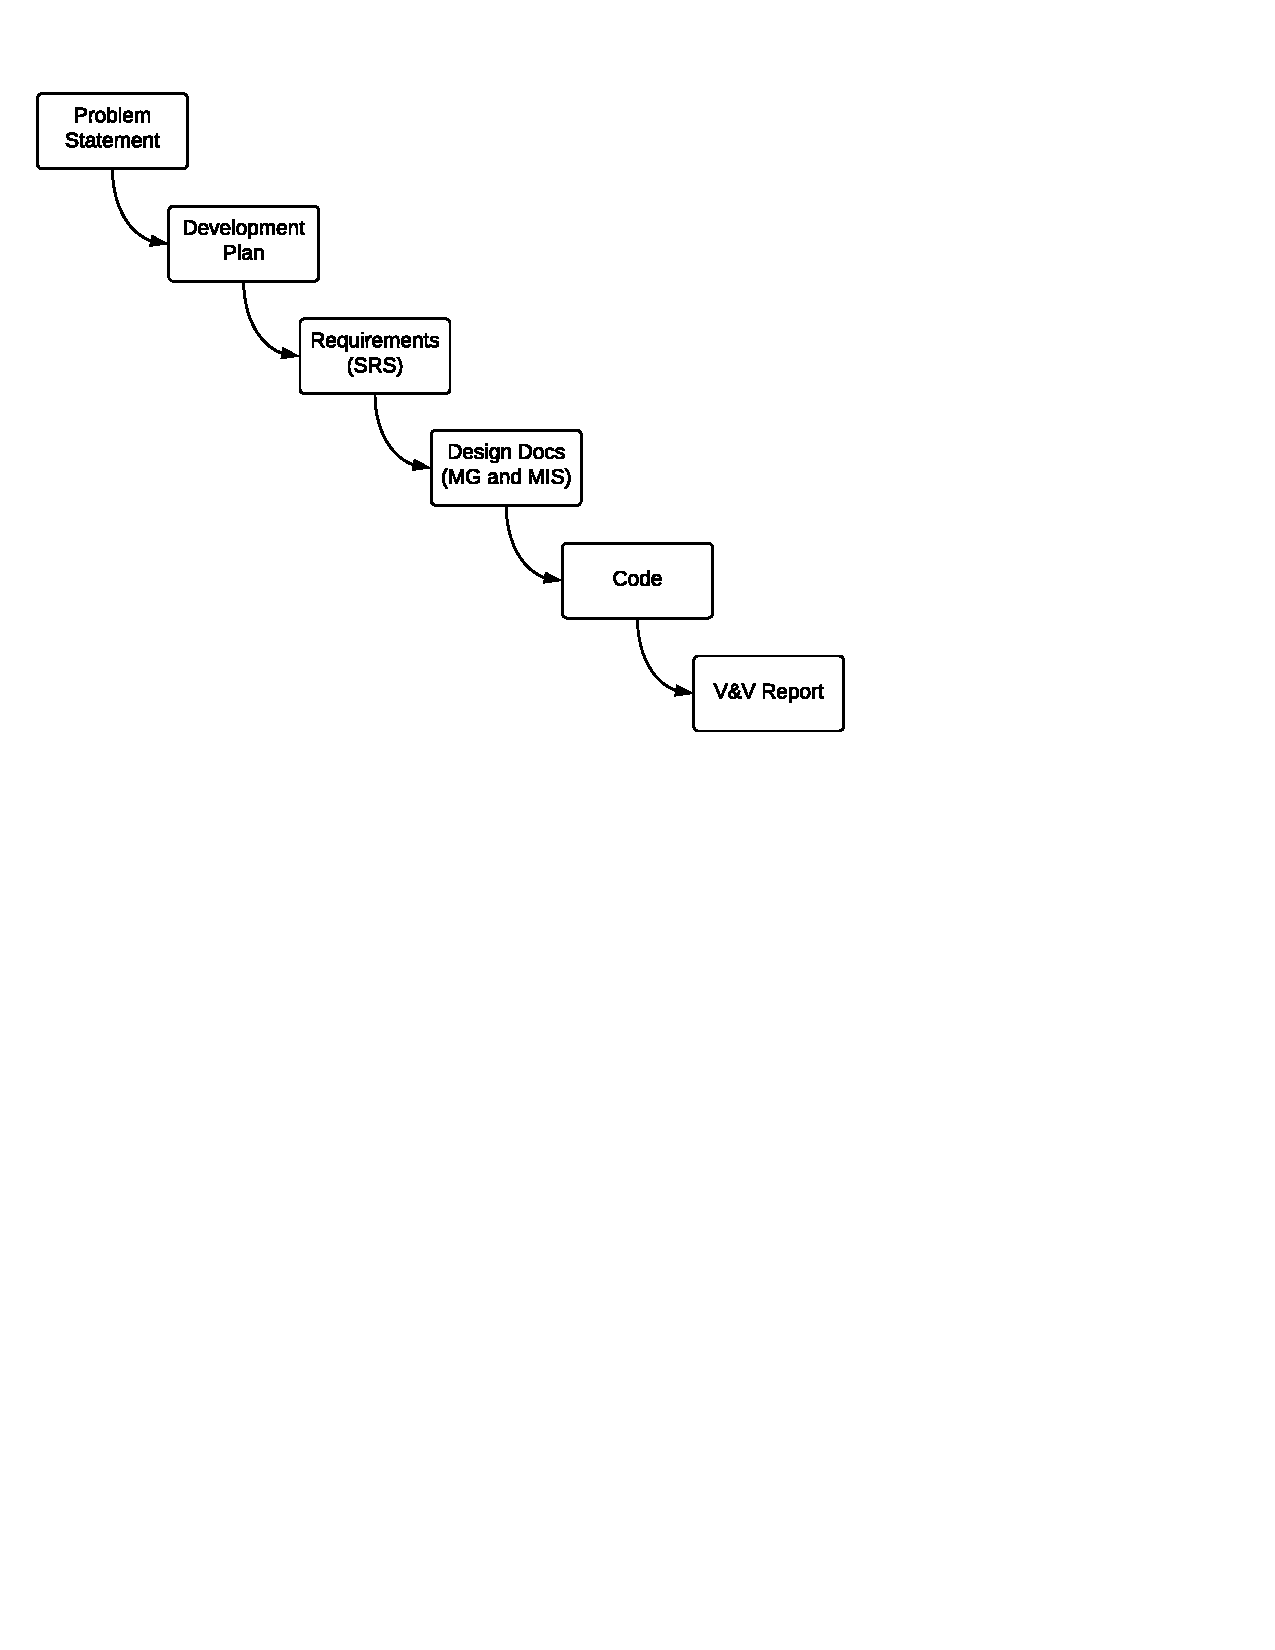
\includegraphics[scale=0.6]{Waterfall.pdf}
\end{center}

SWHS example at
\href{https://github.com/smiths/swhs}{https://github.com/smiths/swhs}

\end{frame}

%%%%%%%%%%%%%%%%%%%%%%%%%%%%%%%%%%%%%%

\hoffset=-.4in %removing side bar for these frames

\begin{frame}[plain, fragile]

%\frametitle{SRS for SWHS}

\begin{center}
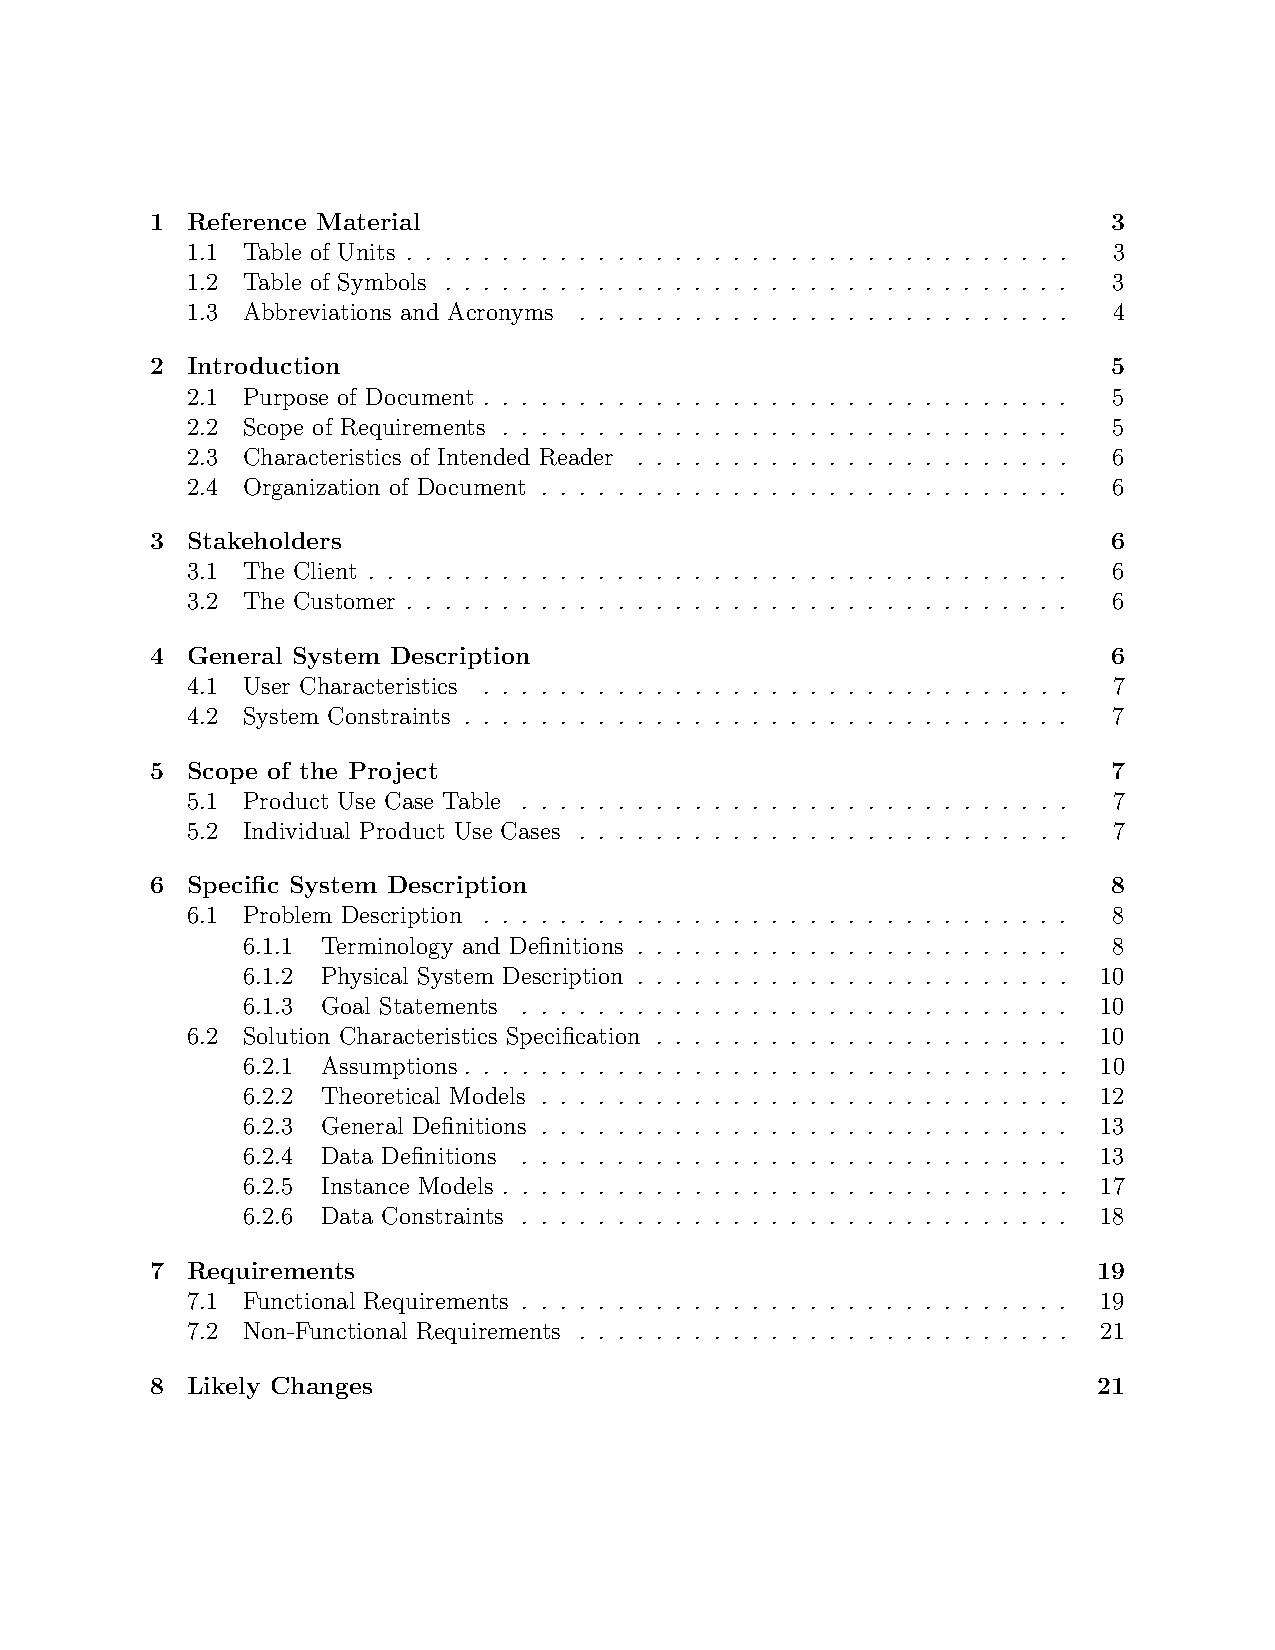
\includegraphics[scale=0.45]{TofC.pdf}
\end{center}

\end{frame}
\hoffset=0in

%%%%%%%%%%%%%%%%%%%%%%%%%%%%%%%%%%%%%%

\begin{frame}

\frametitle{$J_{\mbox{tol}}$ in SRS.pdf}
\begin{center}
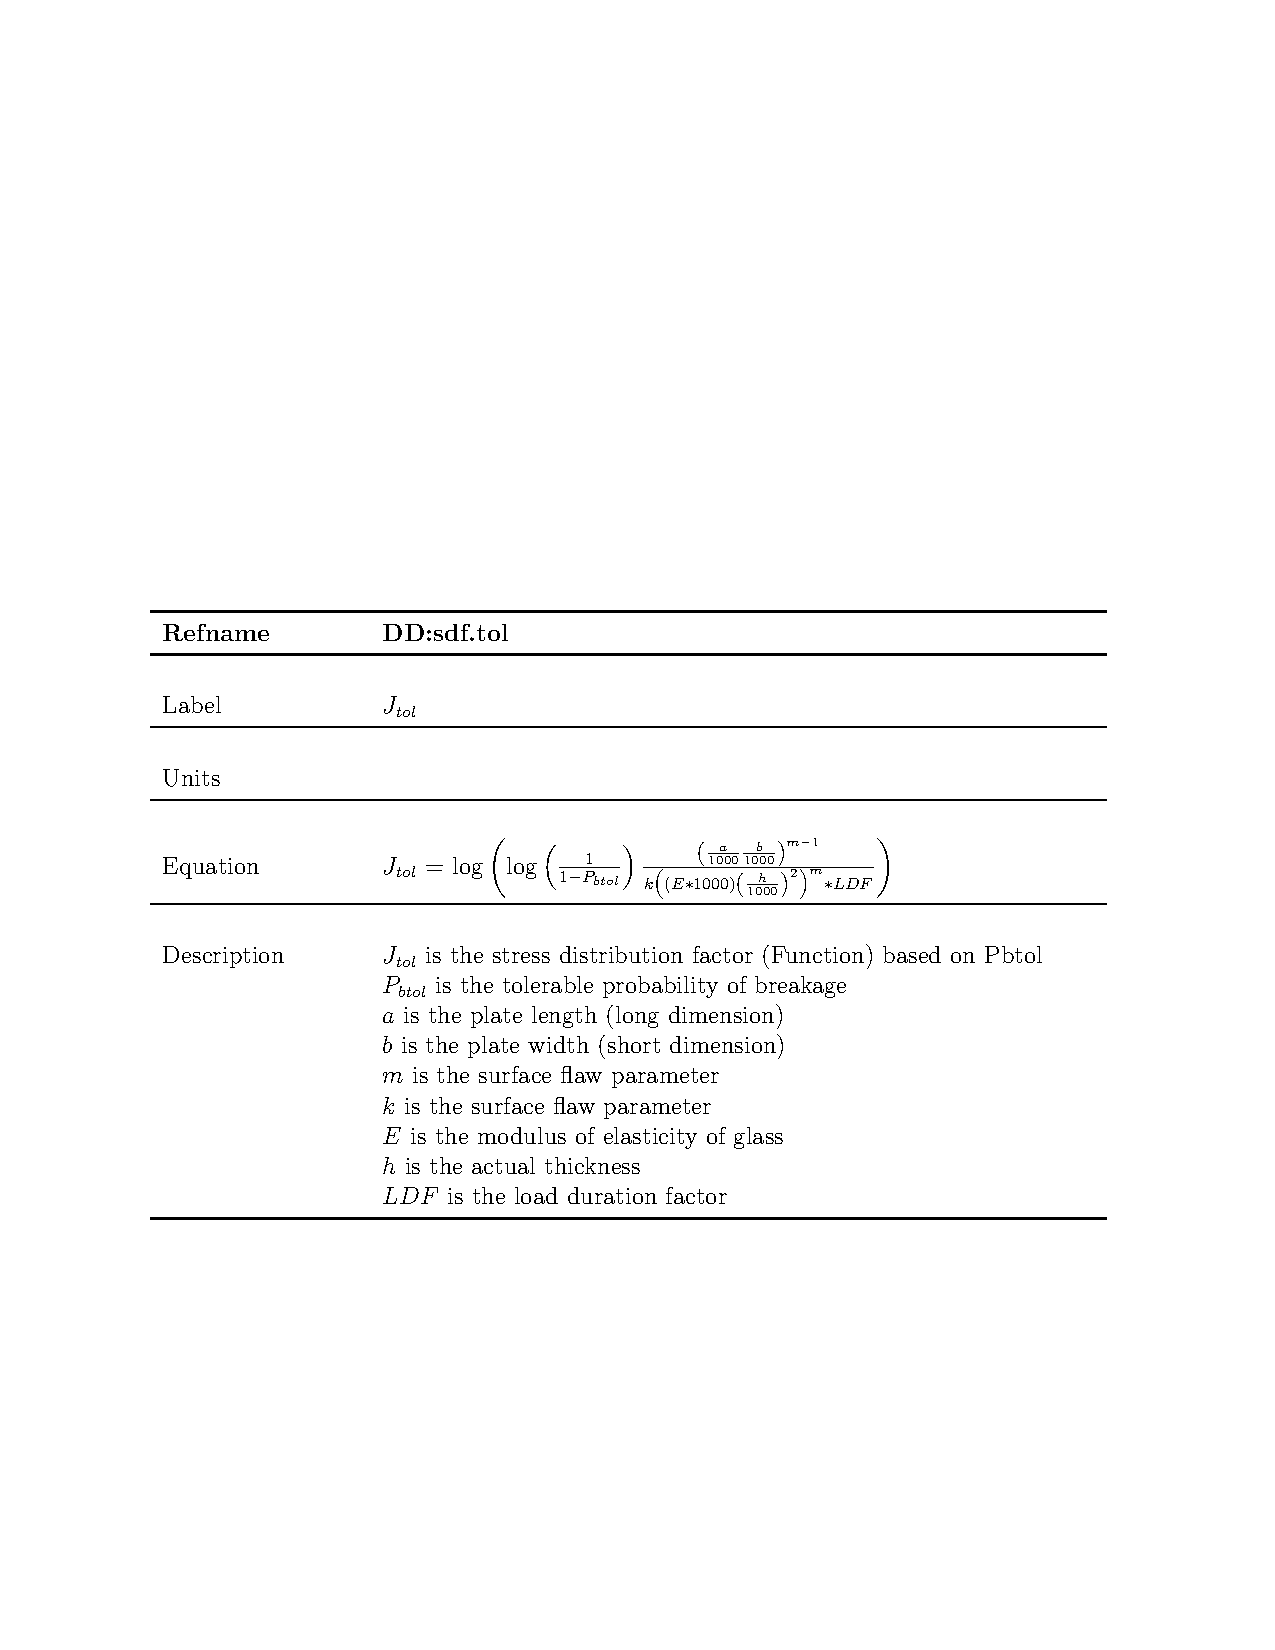
\includegraphics[width=1.0\textwidth]{Jtol_pdf.pdf}
\end{center}
\end{frame}

%%%%%%%%%%%%%%%%%%%%%%%%%%%%%%%%%%%%%

\begin{frame}[plain, fragile]

\frametitle{$J_{\mbox{tol}}$ in SRS.tex}
~\\
\begin{lstlisting}
\noindent \begin{minipage}{\textwidth}
\begin{tabular}{p{0.2\textwidth} p{0.73\textwidth}}
\toprule \textbf{Refname} & \textbf{DD:sdf.tol}
\phantomsection 
\label{DD:sdf.tol}
\\ \midrule \\
Label & $J_{tol}$
\\ \midrule \\
Units & 
\\ \midrule \\
Equation & $J_{tol}$ = $\log\left(\log\left(\frac{1}{1-P_{btol}}\right)\frac{\left(\frac{a}{1000}\frac{b}{1000}\right)^{m-1}}{k\left(\left(E*1000\right)\left(\frac{h}{1000}\right)^{2}\right)^{m}*LDF}\right)$
\\ \midrule \\
Description & $J_{tol}$ is the stress distribution factor (Function) based on
              Pbtol\newline$P_{btol}$ is the tolerable probability of breakage ...
\end{minipage}\\
\end{lstlisting}
\end{frame}

%%%%%%%%%%%%%%%%%%%%%%%%%%%%%%%%%%%%%%

\begin{frame}[plain, fragile]

\frametitle{$J_{\mbox{tol}}$ in SRS.html}

\begin{lstlisting}

<a id="">
<div class="equation">
<em>J<sub>tol</sub></em> = log(log(<div class="fraction">
<span class="fup">
1
</span>
<span class="fdn">
1 &minus; <em>P<sub>btol</sub></em>
</span>
</div>)<div class="fraction">
<span class="fup">
(<div class="fraction">
<span class="fup">
<em>a</em>
</span>
<span class="fdn">
1000
</span>
</div><div class="fraction">
...
\end{lstlisting}

\end{frame}
%%%%%%%%%%%%%%%%%%%%%%%%%%%%%%%%%%%%%

\begin{frame}[plain, fragile]

\frametitle{$J_{\mbox{tol}}$ in Python}

\begin{lstlisting}
def calc_j_tol(inparams):
    j_tol = math.log((math.log(1.0 / (1.0 - inparams.pbtol))) * ((((inparams.a / 1000.0) * (inparams.b / 1000.0)) ** (inparams.m - 1.0)) / ((inparams.k * (((inparams.E * 1000.0) * ((inparams.h / 1000.0) ** 2.0)) ** inparams.m)) * inparams.ldf)))
    return j_tol
\end{lstlisting}
\end{frame}

%%%%%%%%%%%%%%%%%%%%%%%%%%%%%%%%%%%%%%

\begin{frame}[plain, fragile]

\frametitle{$J_{\mbox{tol}}$ in Java}

\begin{lstlisting}
public static double calc_j_tol(InputParameters inparams) {
        double j_tol = Math.log((Math.log(1.0 / (1.0 - inparams.pbtol))) * ((Math.pow((inparams.a / 1000.0) * (inparams.b / 1000.0), inparams.m - 1.0)) / ((inparams.k * (Math.pow((inparams.E * 1000.0) * (Math.pow(inparams.h / 1000.0, 2.0)), inparams.m))) * inparams.ldf)));
        return j_tol;
    }
\end{lstlisting}
\end{frame}

%%%%%%%%%%%%%%%%%%%%%%%%%%%%%%%%%%%%%%

\hoffset=-.7in 
\begin{frame}[plain, fragile]
\frametitle{Code with Comments}
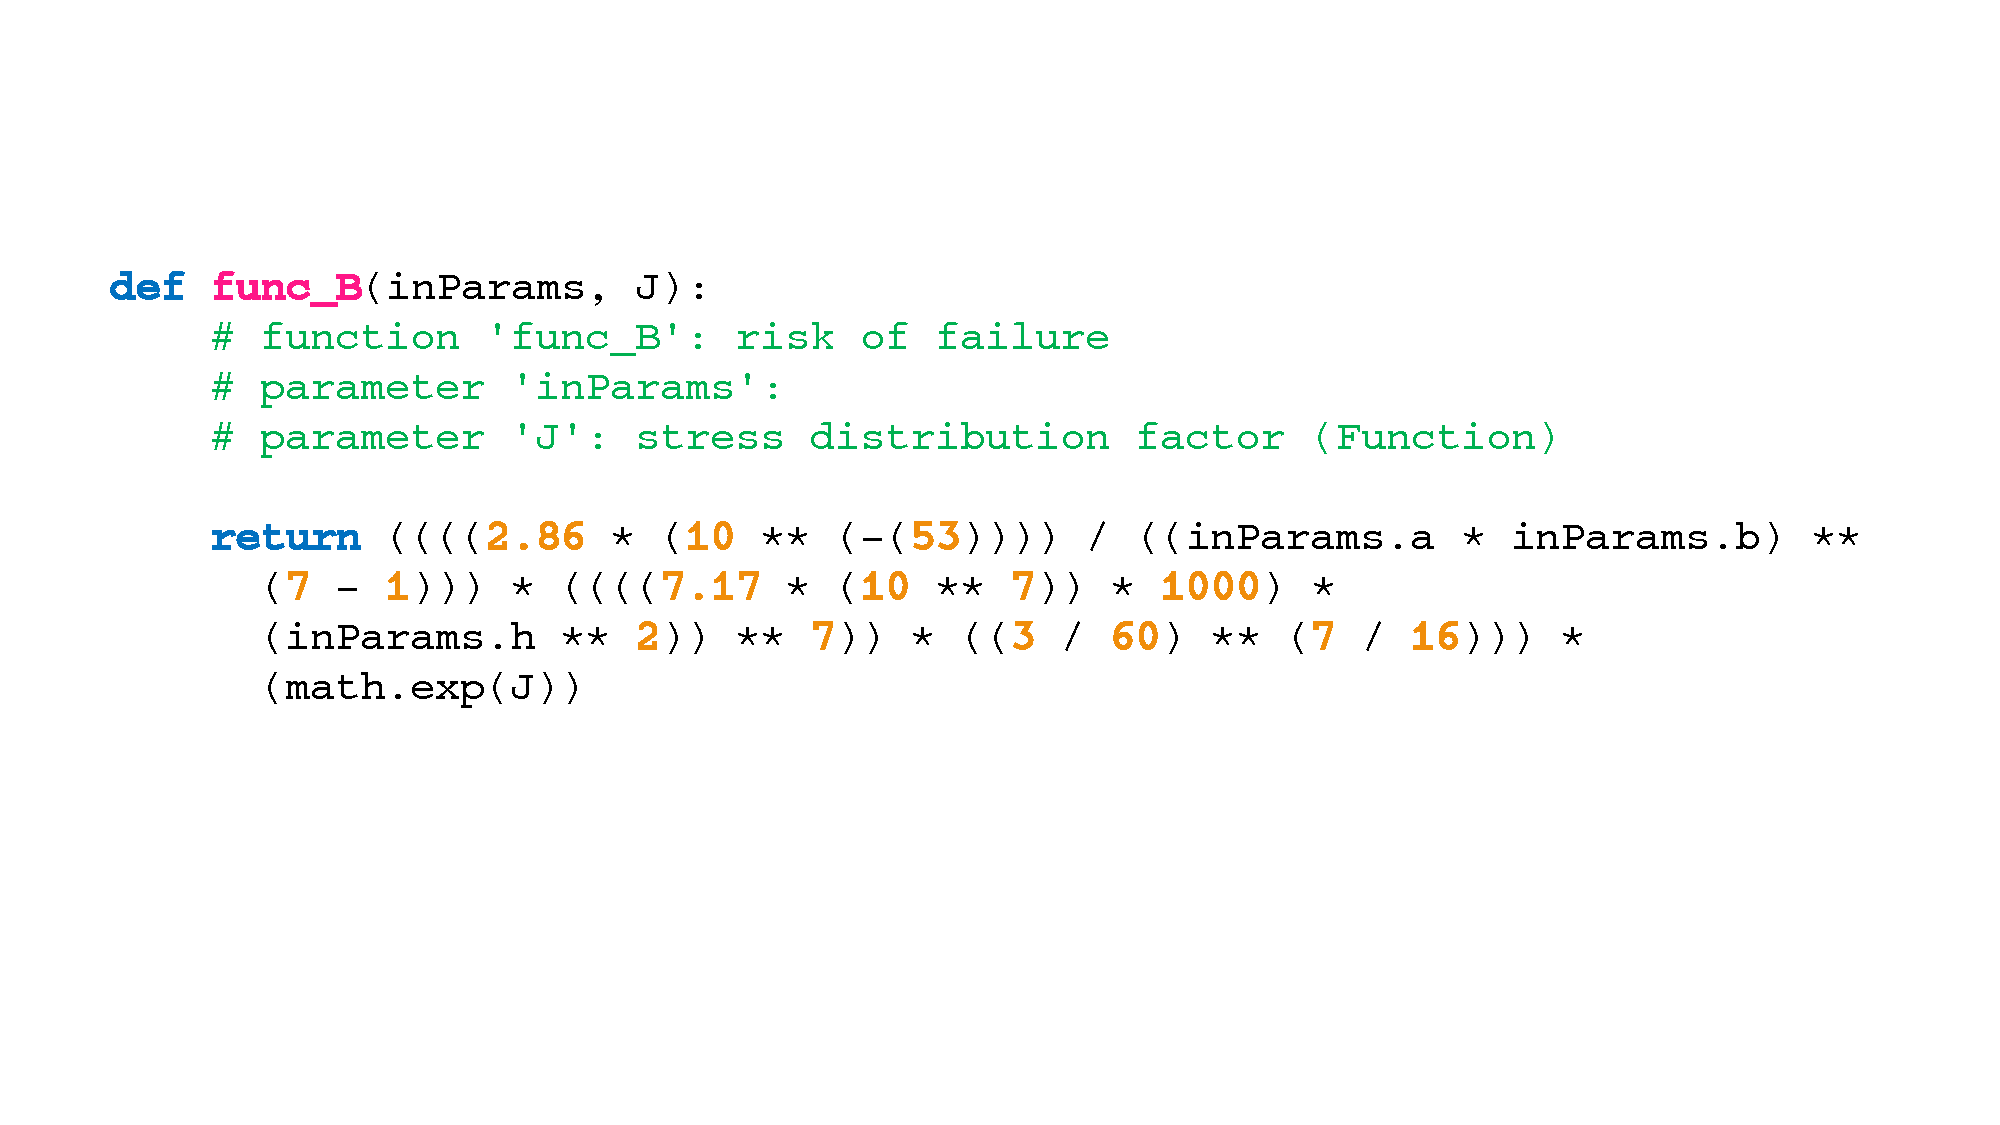
\includegraphics[width=1.2\textwidth]{CommentingOn.pdf}
\end{frame}
\hoffset=0in

%%%%%%%%%%%%%%%%%%%%%%%%%%%%%%%%%%%%%

\hoffset=-.7in 
\begin{frame}[plain, fragile]
\frametitle{Code with Logging}
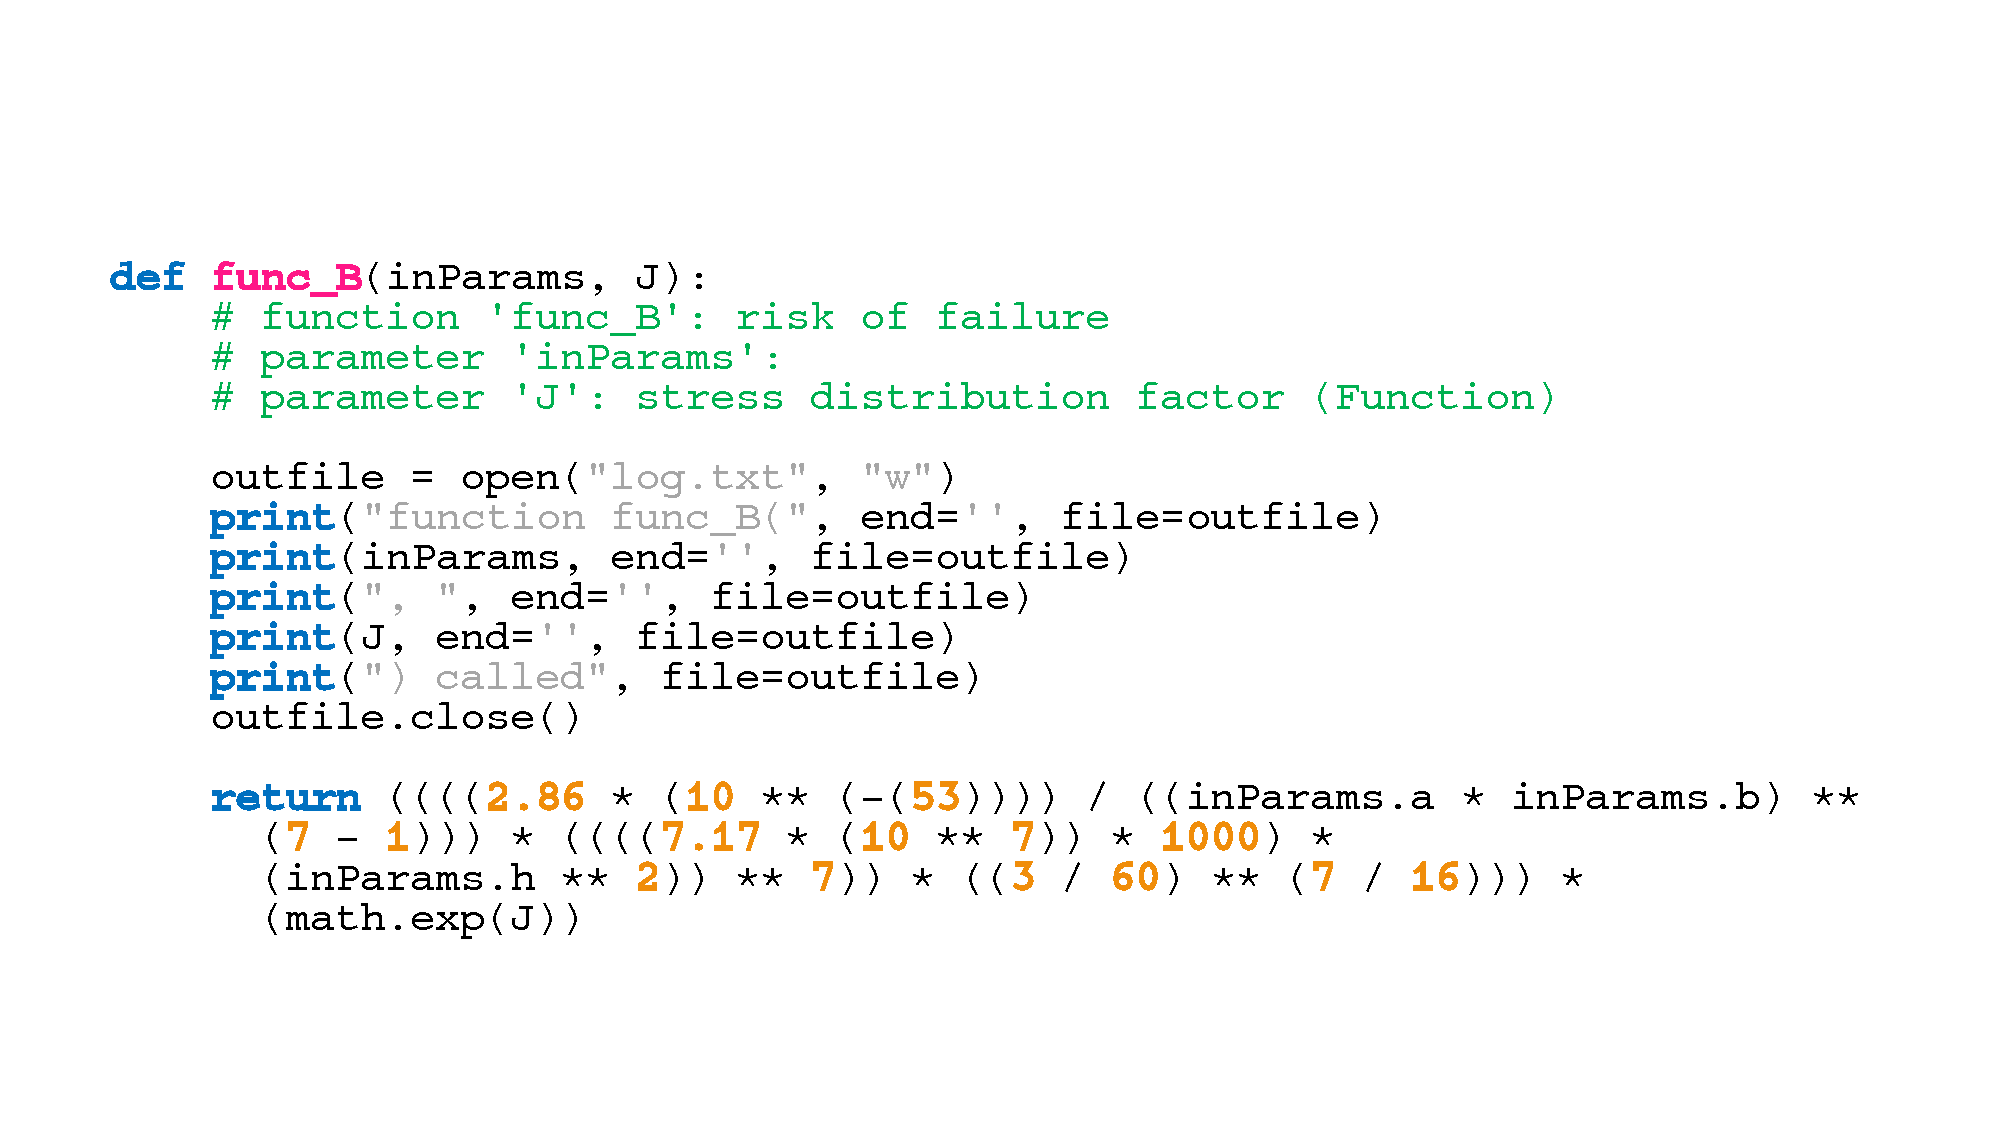
\includegraphics[width=1.2\textwidth]{LoggingOn.pdf}
\end{frame}
\hoffset=0in

%%%%%%%%%%%%%%%%%%%%%%%%%%%%%%%%%%%%%

\begin{frame}[plain, fragile]

\frametitle{$J_{\mbox{tol}}$ in Drasil (Haskell)}

\begin{lstlisting}

tolStrDisFac_eq :: Expr
tolStrDisFac_eq = ln (ln (1 / (1 - (sy pb_tol)))
  * (((((sy plate_len)/1000.0) * ((sy plate_width)/1000.0)) $^ (sy sflawParamM - 1) / 
    ((sy sflawParamK) * (((sy mod_elas * 1000.0) *
    (square ((sy min_thick)/1000.0))))) $^ (sy sflawParamM) * (sy lDurFac)))))

\end{lstlisting}
\end{frame}

%%%%%%%%%%%%%%%%%%%%%%%%%%%%%%%%%%%%%%

\begin{frame}[plain, fragile]

\frametitle{$J_{\mbox{tol}}$ without Unit Conversion}

\begin{lstlisting}
tolStrDisFac_eq :: Expr
tolStrDisFac_eq = ln (ln (1 / (1 - (sy pb_tol)))
  * ((((sy plate_len) * (sy plate_width)) $^ (sy sflawParamM - 1) / 
    ((sy sflawParamK) * ((sy mod_elas *
    (square (sy min_thick)))) $^ (sy sflawParamM) * (sy lDurFac)))))
\end{lstlisting}
\end{frame}

%%%%%%%%%%%%%%%%%%%%%%%%%%%%%%%%%%%%%%

\hoffset=-.7in 
\begin{frame}[plain, fragile]
\frametitle{Complete and Consistent}
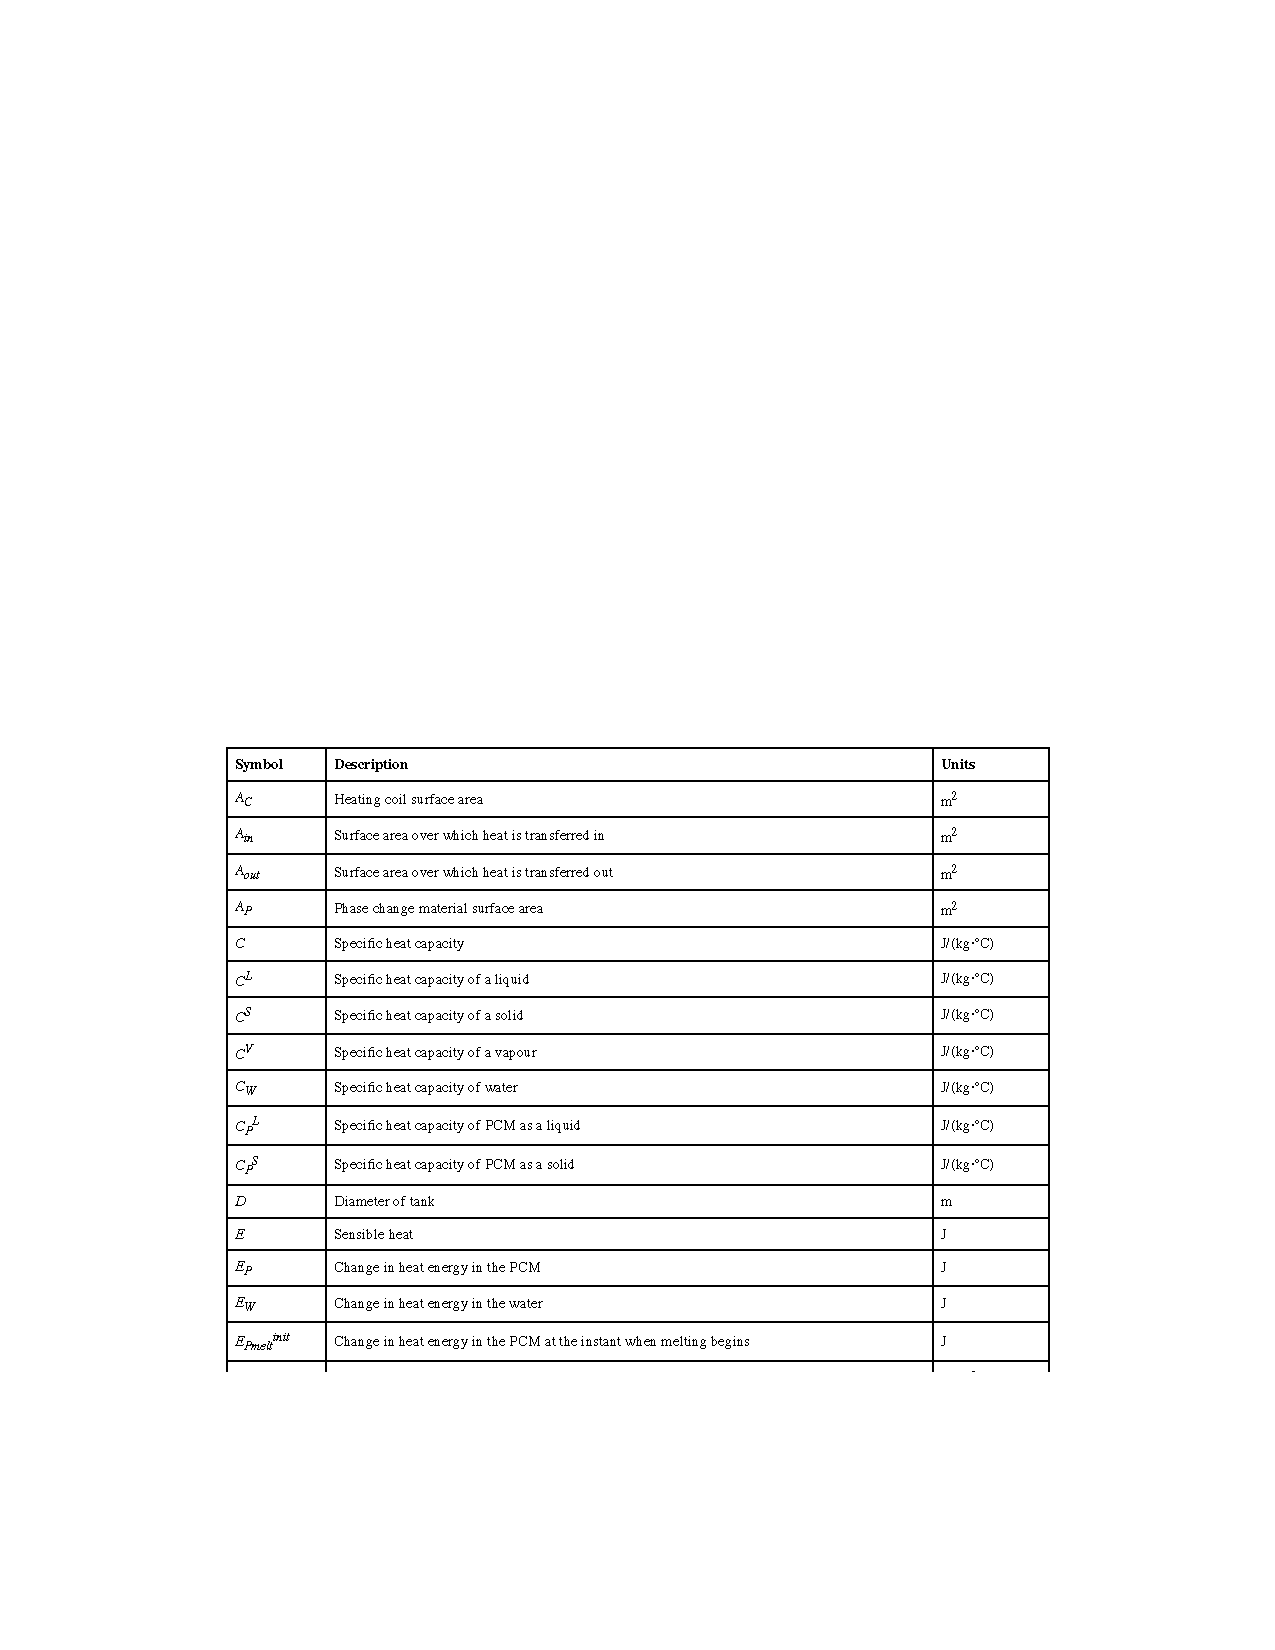
\includegraphics[width=1.2\textwidth]{TableOfSymbols.pdf}
\end{frame}
\hoffset=0in

%%%%%%%%%%%%%%%%%%%%%%%%%%%%%%%%%%%%%

\hoffset=-.7in 
\begin{frame}[plain, fragile]
\frametitle{Complete and Consistent Cont'd}
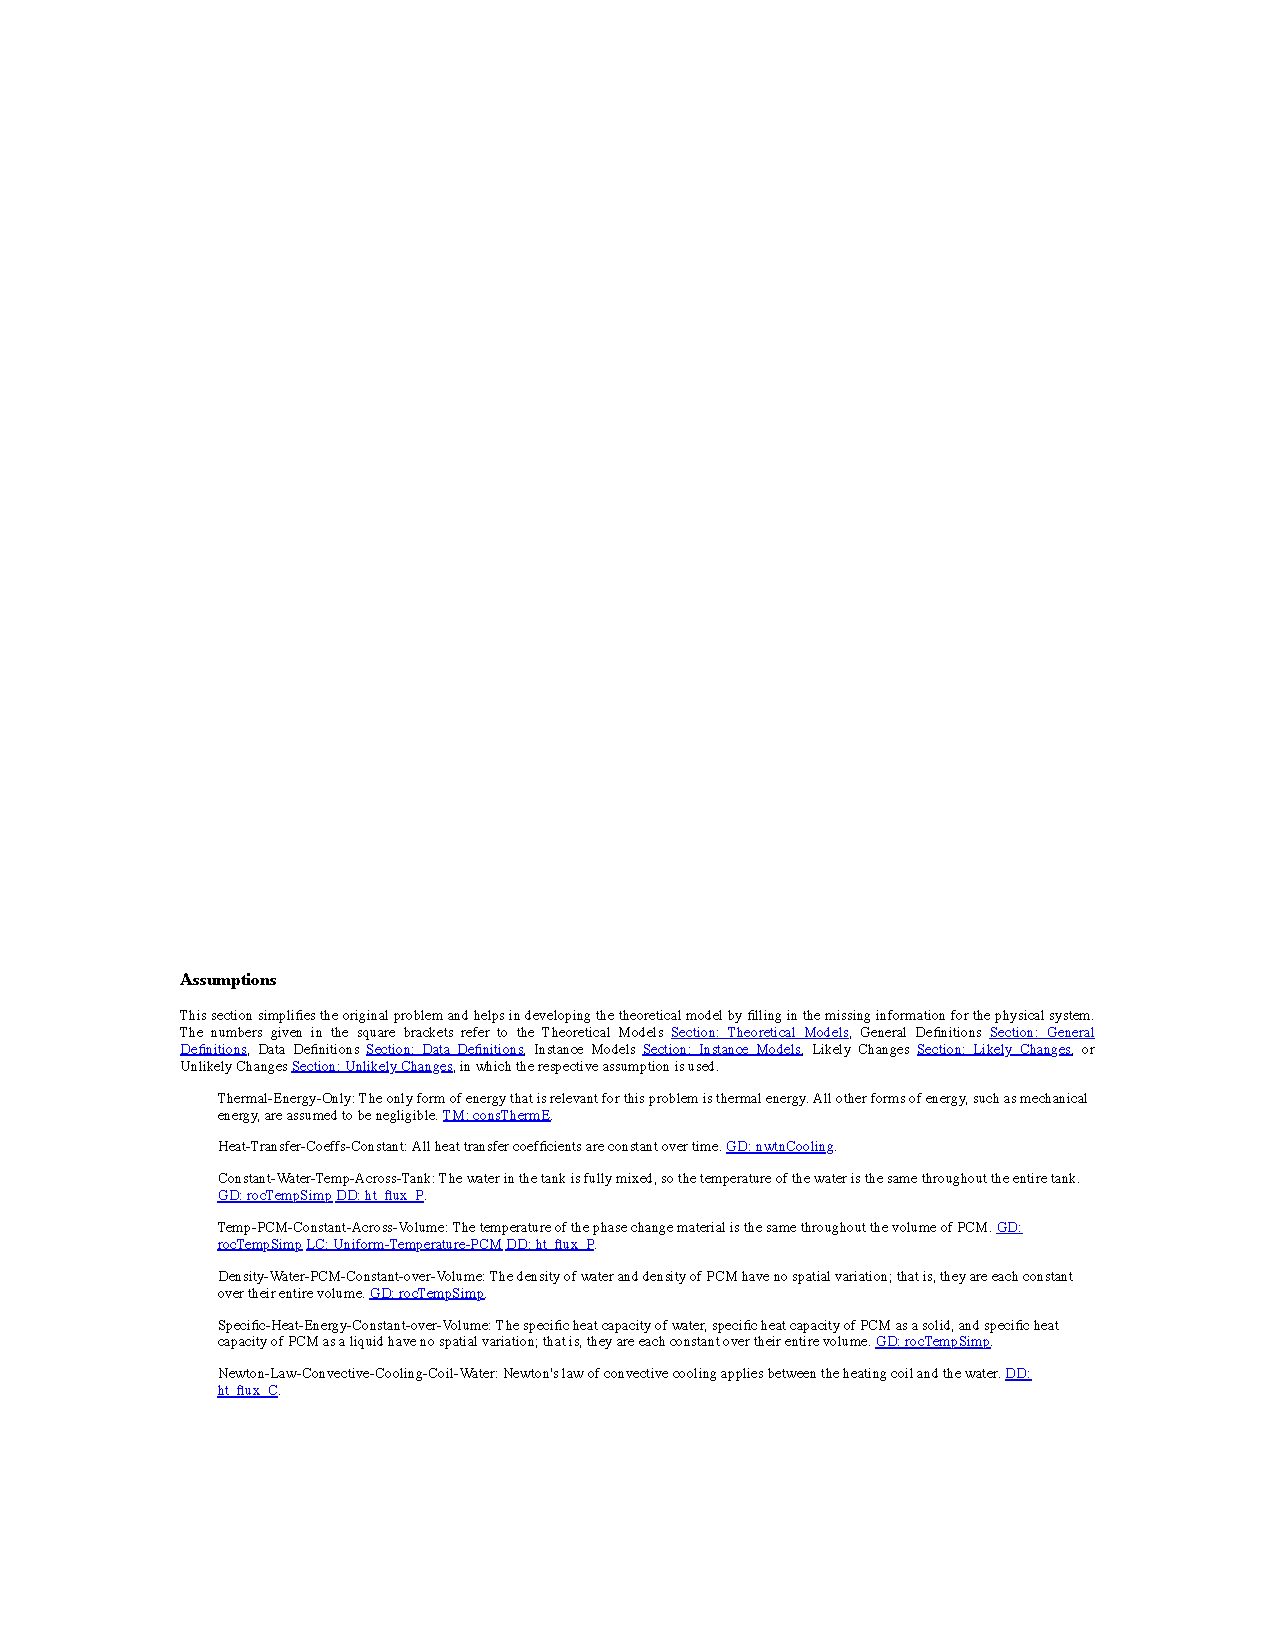
\includegraphics[width=1.2\textwidth]{Assumptions.pdf}
\end{frame}
\hoffset=0in

%%%%%%%%%%%%%%%%%%%%%%%%%%%%%%%%%%%%%

\hoffset=-.7in %removing side bar for these frames
\begin{frame}[plain, fragile]

\frametitle{Traceability Graph}

\begin{center}
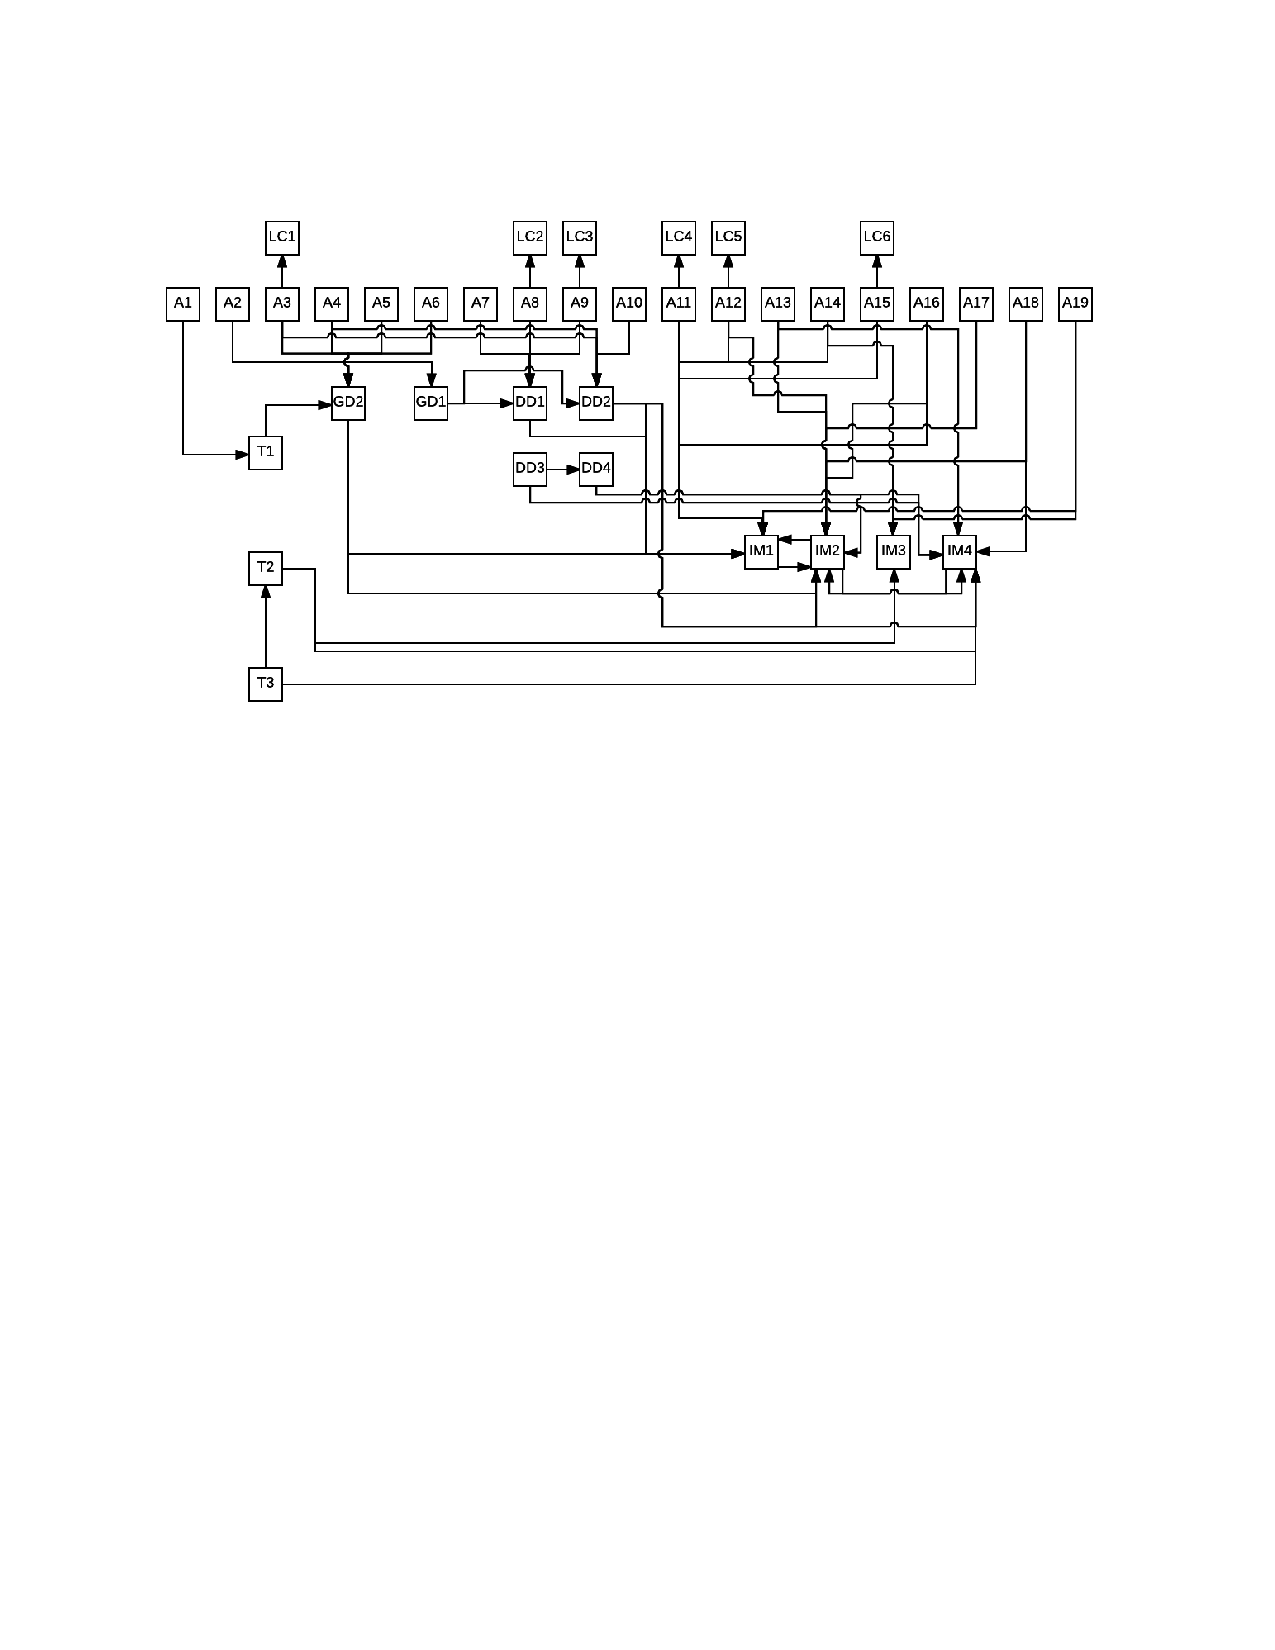
\includegraphics[scale=0.75]{TraceGraph.pdf}
\end{center}

\end{frame}
\hoffset=0in

%%%%%%%%%%%%%%%%%%%%%%%%%%%%%%%%%%%%%%

\end{document}